\documentclass[12pt]{article}
\usepackage{amsmath, amssymb, amsthm}
\usepackage{enumitem}
\usepackage[hidelinks]{hyperref}
\usepackage{tikz}
\usetikzlibrary{positioning, shapes, arrows.meta, calc, patterns}

% Theorem environments
\newtheorem{theorem}{Theorem}[section]
\newtheorem{lemma}[theorem]{Lemma} 
\newtheorem{corollary}[theorem]{Corollary}

\theoremstyle{definition}
\newtheorem{definition}[theorem]{Definition}
\newtheorem{example}[theorem]{Example}

\begin{document}

\title{Discrete Mathematics: Conceptual Insights and Advanced Formulas}
\author{}
\date{\today}
\maketitle

\tableofcontents

%%%%%%%%%%%%%%%%%%%%%%%%%%%%%%%%%%%%%%%%%%%%%%%%%%%%%%%%%%%%%%%%%%%%%
\section{Introduction and Fundamental Concepts}

Discrete mathematics forms the backbone of computer science, cryptography, and combinatorial optimization. Its language—sets, functions, relations, and counting—is essential for structuring rigorous arguments and designing algorithms. In these notes, we present definitions and theorems while discussing the ideas behind them and illustrating concepts with diagrams.

%%%%%%%%%%%%%%%%%%%%%%%%%%%%%%%%%%%%%%%%%%%%%%%%%%%%%%%%%%%%%%%%%%%%%
\subsection{Numbers and Sets: Notation and Concepts}

Understanding number systems and set theory is critical because they provide the basic vocabulary for nearly every mathematical discussion.

\begin{definition}[Common Number Sets]
  \begin{itemize}[itemsep=3pt]
    \item \(\mathbb{N}\): the set of \emph{natural numbers}. (Note: Some define \(\mathbb{N}=\{0,1,2,\dots\}\), others \(\{1,2,\dots\}\).)
    \item \(\mathbb{Z}\): the set of \emph{integers}: \(\{ \dots, -2, -1, 0, 1, 2, \dots \}\).
    \item \(\mathbb{Q}\): the set of \emph{rational numbers}.
    \item \(\mathbb{R}\): the set of \emph{real numbers}.
    \item \(\mathbb{C}\): the set of \emph{complex numbers}.
  \end{itemize}
  \vspace{0.5em}
  \textbf{Why It Matters:} Each number set expands the types of problems you can solve. For example, \(\mathbb{N}\) underpins counting, while \(\mathbb{R}\) allows us to model continuous change.
\end{definition}

% Diagram: Nested number sets
\begin{center}
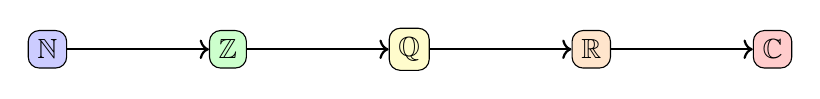
\begin{tikzpicture}[node distance=1.8cm, auto]
  \node[draw, rectangle, rounded corners, fill=blue!20] (N) {\(\mathbb{N}\)};
  \node[draw, rectangle, rounded corners, fill=green!20, right=of N] (Z) {\(\mathbb{Z}\)};
  \node[draw, rectangle, rounded corners, fill=yellow!20, right=of Z] (Q) {\(\mathbb{Q}\)};
  \node[draw, rectangle, rounded corners, fill=orange!20, right=of Q] (R) {\(\mathbb{R}\)};
  \node[draw, rectangle, rounded corners, fill=red!20, right=of R] (C) {\(\mathbb{C}\)};
  \draw[->, thick] (N) -- (Z);
  \draw[->, thick] (Z) -- (Q);
  \draw[->, thick] (Q) -- (R);
  \draw[->, thick] (R) -- (C);
\end{tikzpicture}
\end{center}

\begin{definition}[Basic Set Notation]
  A \emph{set} is a collection of distinct objects. We denote a set as
  \[
  A = \{ a, b, c, \dots \},
  \]
  and write \(a \in A\) if \(a\) is an element of \(A\). Important notations include:
  \begin{itemize}[itemsep=3pt]
    \item \(|A|\): the \emph{cardinality} (number of elements in \(A\)).
    \item \(A \subseteq B\): \(A\) is a \emph{subset} of \(B\).
    \item \(A \cup B\): the \emph{union} of \(A\) and \(B\).
    \item \(A \cap B\): the \emph{intersection} of \(A\) and \(B\).
    \item \(A \setminus B\): the \emph{set difference}.
    \item \(A^c\) or \(\overline{A}\): the \emph{complement} of \(A\) (relative to a universal set \(U\)).
    \item \(\mathcal{P}(A)\): the \emph{power set} of \(A\), with \(|\mathcal{P}(A)| = 2^{|A|}\) when \(A\) is finite.
  \end{itemize}
  \vspace{0.5em}
  \textbf{Why It Matters:} Mastering set operations is essential for formal proofs, algorithm design, and understanding data structures.
\end{definition}

% Diagram: Venn diagram for union, intersection, and complement
\begin{center}
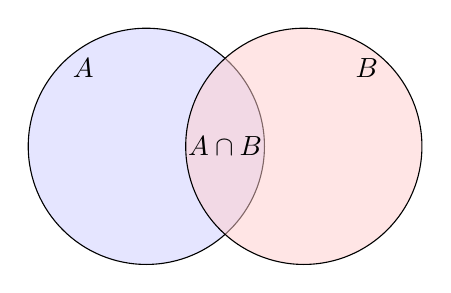
\begin{tikzpicture}
  % Draw two overlapping circles
  \draw[fill=blue!20, fill opacity=0.5] (0,0) circle (1.5);
  \draw[fill=red!20, fill opacity=0.5] (2,0) circle (1.5);
  % Label the sets
  \node at (-0.8,1) {\(A\)};
  \node at (2.8,1) {\(B\)};
  \node at (1,0) {\(A\cap B\)};
\end{tikzpicture}
\end{center}

\begin{lemma}[De Morgan's Laws]
  For any two sets \(A\) and \(B\) (with respect to a universal set \(U\)):
  \[
  (A \cup B)^c = A^c \cap B^c \quad \text{and} \quad (A \cap B)^c = A^c \cup B^c.
  \]
  \vspace{0.5em}
  \textbf{Conceptual Insight:} These laws show the duality between union and intersection under complementation.
\end{lemma}

% Diagram: Venn diagram illustrating De Morgan's Laws
\begin{center}
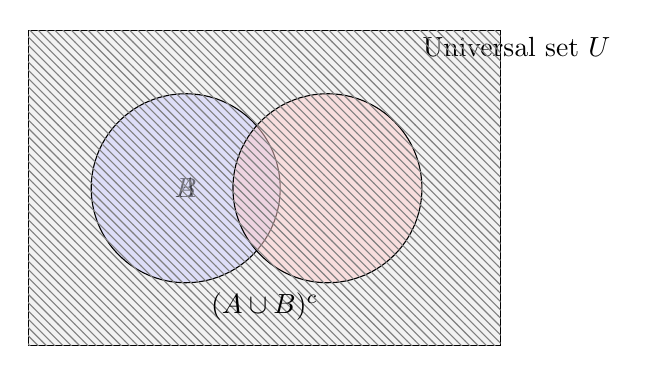
\begin{tikzpicture}
  % Universal set
  \draw[fill=gray!10] (-2,-2) rectangle (4,2);
  \node at (4.2,1.8) {Universal set \(U\)};
  % Circles for A and B
  \draw[fill=blue!20, fill opacity=0.5] (0,0) circle (1.2) node[pos=0.5] {\(A\)};
  \draw[fill=red!20, fill opacity=0.5] (1.8,0) circle (1.2) node[pos=0.5] {\(B\)};
  % Shade (A U B)^c
  \begin{scope}
    \clip (-2,-2) rectangle (4,2);
    \fill[pattern=north west lines, pattern color=black!50] (-2,-2) rectangle (4,2);
    \clip (0,0) circle (1.2);
    \clip (1.8,0) circle (1.2);
  \end{scope}
  \node at (1,-1.5) {\((A\cup B)^c\)};
\end{tikzpicture}
\end{center}

%%%%%%%%%%%%%%%%%%%%%%%%%%%%%%%%%%%%%%%%%%%%%%%%%%%%%%%%%%%%%%%%%%%%%
\subsection{Mathematical Induction and Other Proof Techniques}

Mathematical induction is like a row of dominos: if the first falls (the base case) and every domino knocks over the next (the inductive step), then the entire row falls (the statement holds for all natural numbers).

\begin{theorem}[Principle of Mathematical Induction]
  Let \(P(n)\) be a proposition about \(n \in \mathbb{N}\). If:
  \begin{enumerate}[label=(\roman*)]
    \item \textbf{Base Case:} \(P(1)\) is true.
    \item \textbf{Inductive Step:} For every \(k \in \mathbb{N}\), \(P(k)\) true implies \(P(k+1)\) is true.
  \end{enumerate}
  Then \(P(n)\) is true for all \(n \in \mathbb{N}\).
  \vspace{0.5em}
  \textbf{Why It Matters:} Induction is essential for proving infinite families of statements—a technique central to algorithm correctness and number theory.
\end{theorem}

% Diagram: Flowchart of induction
\begin{center}
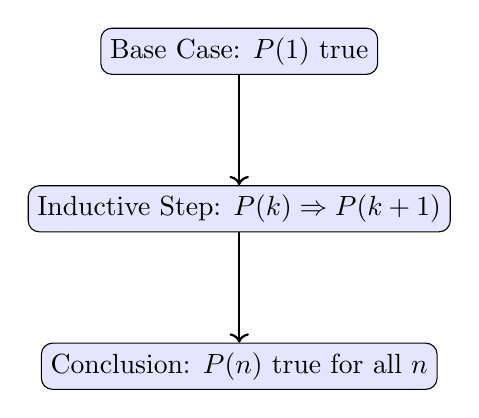
\begin{tikzpicture}[node distance=2cm, auto, every node/.style={draw, rectangle, rounded corners, fill=blue!10}]
  \node (base) {Base Case: \(P(1)\) true};
  \node (inductive) [below of=base] {Inductive Step: \(P(k) \Rightarrow P(k+1)\)};
  \node (conclusion) [below of=inductive] {Conclusion: \(P(n)\) true for all \(n\)};
  \draw[->, thick] (base) -- (inductive);
  \draw[->, thick] (inductive) -- (conclusion);
\end{tikzpicture}
\end{center}

\begin{theorem}[Principle of Strong Induction]
  Let \(P(n)\) be a proposition about \(n \in \mathbb{N}\). If:
  \begin{enumerate}[label=(\roman*)]
    \item \textbf{Base Case:} \(P(1)\) is true.
    \item \textbf{Inductive Step:} For all \(n \ge 1\), if \(P(1), P(2), \dots, P(n)\) are true, then \(P(n+1)\) is true.
  \end{enumerate}
  Then \(P(n)\) is true for all \(n \in \mathbb{N}\).
  \vspace{0.5em}
  \textbf{Conceptual Note:} Strong induction is particularly useful when \(P(n+1)\) depends on several previous cases.
\end{theorem}

\begin{example}[Prime Factorization]
  \textbf{Statement:} Every integer \(n > 1\) can be written as a product of primes.
  
  \textbf{Proof (by strong induction):}
  \begin{itemize}[itemsep=3pt]
    \item \emph{Base Case:} \(n = 2\) is prime.
    \item \emph{Inductive Step:} Assume every integer \(2 \le k \le n\) can be factored into primes. For \(n+1\): if it is prime, we are done; if composite, write \(n+1 = ab\) with \(2 \le a,b \le n\). Then, by the induction hypothesis, both \(a\) and \(b\) have prime factorizations, so \(n+1\) does as well.
  \end{itemize}
  \vspace{0.5em}
  \textbf{Why It Matters:} This proof underpins the Fundamental Theorem of Arithmetic.
\end{example}

%%%%%%%%%%%%%%%%%%%%%%%%%%%%%%%%%%%%%%%%%%%%%%%%%%%%%%%%%%%%%%%%%%%%%
\subsection{Functions}

Functions formalize the idea of a rule mapping inputs to outputs, which is vital in modeling processes and computer algorithms.

\begin{definition}[Function]
  A \emph{function} \(f\) from a set \(A\) to a set \(B\), written \(f: A \to B\), assigns each \(a \in A\) a unique element \(f(a) \in B\). Here:
  \begin{itemize}[itemsep=3pt]
    \item \(A\) is the \emph{domain}.
    \item \(B\) is the \emph{codomain}.
    \item The \emph{image} of \(f\) is \(\{ f(a) \mid a \in A \}\).
  \end{itemize}
  \vspace{0.5em}
  \textbf{Why It Matters:} Functions are central to describing processes and are the building blocks of mathematical modeling.
\end{definition}

% Diagram: Mapping from A to B
\begin{center}
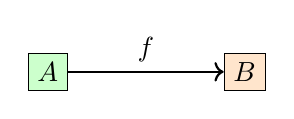
\begin{tikzpicture}[node distance=2.5cm, auto]
  \node[draw, rectangle, fill=green!20] (A) {\(A\)};
  \node[draw, rectangle, fill=orange!20] (B) [right of=A] {\(B\)};
  \draw[->, thick] (A) -- node[midway, above] {\(f\)} (B);
\end{tikzpicture}
\end{center}

\begin{definition}[Types of Functions]
  A function \(f: A \to B\) is:
  \begin{itemize}[itemsep=3pt]
    \item \textbf{Injective (one-to-one)}: \(f(a_1)=f(a_2)\) implies \(a_1 = a_2\).
    \item \textbf{Surjective (onto)}: For every \(b \in B\), there exists \(a \in A\) such that \(f(a)=b\).
    \item \textbf{Bijective}: Both injective and surjective.
  \end{itemize}
  \vspace{0.5em}
  \textbf{Conceptual Insight:} Recognizing function types helps determine invertibility and structure in algorithms.
\end{definition}

% Diagram: Composition of functions (A -> B -> C)
\begin{center}
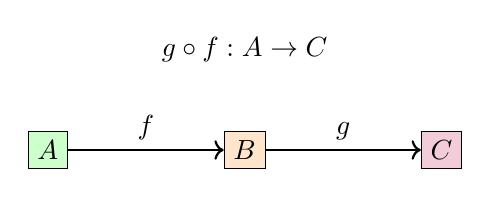
\begin{tikzpicture}[node distance=2.5cm, auto]
  \node[draw, rectangle, fill=green!20] (A) {\(A\)};
  \node[draw, rectangle, fill=orange!20] (B) [right of=A] {\(B\)};
  \node[draw, rectangle, fill=purple!20] (C) [right of=B] {\(C\)};
  \draw[->, thick] (A) -- node[midway, above] {\(f\)} (B);
  \draw[->, thick] (B) -- node[midway, above] {\(g\)} (C);
  \node at ($(A)!0.5!(C)$) [above=1cm] {\(g \circ f: A \to C\)};
\end{tikzpicture}
\end{center}

\begin{lemma}[Composition of Functions]
  Let \(f: A \to B\) and \(g: B \to C\). Then the composition \(g \circ f: A \to C\) defined by
  \[
  (g \circ f)(a) = g(f(a))
  \]
  is a function. Moreover:
  \begin{itemize}
    \item If \(f\) and \(g\) are injective, then \(g \circ f\) is injective.
    \item If \(f\) and \(g\) are surjective, then \(g \circ f\) is surjective.
    \item If \(f\) and \(g\) are bijective, then \(g \circ f\) is bijective with inverse \((g \circ f)^{-1} = f^{-1} \circ g^{-1}\).
  \end{itemize}
  \vspace{0.5em}
  \textbf{Why It Matters:} Composing functions is analogous to chaining processes—a key idea in building complex algorithms from simple modules.
\end{lemma}

%%%%%%%%%%%%%%%%%%%%%%%%%%%%%%%%%%%%%%%%%%%%%%%%%%%%%%%%%%%%%%%%%%%%%
\subsection{Relations}

Relations generalize functions and describe various associations between elements, which are essential in structuring data and logical statements.

\begin{definition}[Relation]
  A \emph{relation} \(R\) on a set \(A\) is a subset of the Cartesian product \(A \times A\):
  \[
  R \subseteq A \times A.
  \]
  If \((a,b) \in R\), we write \(a\,R\,b\).
\end{definition}

\begin{definition}[Properties of Relations]
  Let \(R\) be a relation on \(A\). Then:
  \begin{itemize}[itemsep=3pt]
    \item \(R\) is \emph{reflexive} if \(a\,R\,a\) for every \(a \in A\).
    \item \(R\) is \emph{symmetric} if \(a\,R\,b\) implies \(b\,R\,a\) for all \(a,b \in A\).
    \item \(R\) is \emph{antisymmetric} if \(a\,R\,b\) and \(b\,R\,a\) imply \(a = b\).
    \item \(R\) is \emph{transitive} if \(a\,R\,b\) and \(b\,R\,c\) imply \(a\,R\,c\) for all \(a,b,c \in A\).
  \end{itemize}
  \vspace{0.5em}
  \textbf{Why It Matters:} These properties help classify relations (like orders or equivalence relations) that are central to database theory and logic.
\end{definition}

% Diagram: Directed graph showing a symmetric relation
\begin{center}
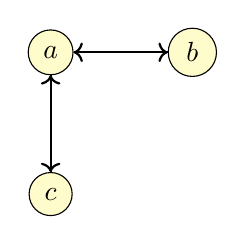
\begin{tikzpicture}[node distance=1.8cm, auto]
  \node[draw, circle, fill=yellow!20] (a) {\(a\)};
  \node[draw, circle, fill=yellow!20] (b) [right of=a] {\(b\)};
  \node[draw, circle, fill=yellow!20] (c) [below of=a] {\(c\)};
  \draw[->, thick] (a) -- (b);
  \draw[->, thick] (b) -- (a);
  \draw[->, thick] (a) -- (c);
  \draw[->, thick] (c) -- (a);
\end{tikzpicture}
\end{center}

\begin{lemma}[Composition of Relations]
  If \(R\) and \(S\) are relations on \(A\), their composition is:
  \[
  R \circ S = \{ (a,c) \in A \times A \mid \exists\, b \in A \text{ with } (a,b) \in S \text{ and } (b,c) \in R \}.
  \]
  \vspace{0.5em}
  \textbf{Conceptual Note:} Composing relations is analogous to linking steps in a process, useful in graph theory and state-transition analysis.
\end{lemma}

%%%%%%%%%%%%%%%%%%%%%%%%%%%%%%%%%%%%%%%%%%%%%%%%%%%%%%%%%%%%%%%%%%%%%
\subsection{Equivalence Relations and Partitions}

Equivalence relations group elements into classes based on a shared property, simplifying analysis by reducing redundancy.

\begin{definition}[Equivalence Relation]
  A relation \(R\) on a set \(A\) is an \emph{equivalence relation} if it is reflexive, symmetric, and transitive.
  \vspace{0.5em}
  \textbf{Why It Matters:} Equivalence relations partition a set into disjoint equivalence classes—a key concept in modular arithmetic and classification problems.
\end{definition}

% Diagram: Partitioning a set into equivalence classes
\begin{center}
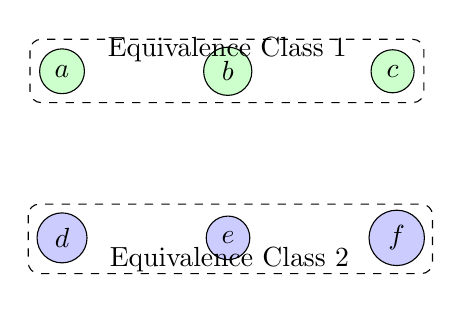
\begin{tikzpicture}[node distance=1.5cm, auto]
  \node[draw, circle, fill=green!20] (a1) {\(a\)};
  \node[draw, circle, fill=green!20] (a2) [right=of a1] {\(b\)};
  \node[draw, circle, fill=green!20] (a3) [right=of a2] {\(c\)};
  \node[draw, circle, fill=blue!20] (b1) [below=of a1] {\(d\)};
  \node[draw, circle, fill=blue!20] (b2) [right=of b1] {\(e\)};
  \node[draw, circle, fill=blue!20] (b3) [right=of b2] {\(f\)};
  \draw[dashed, rounded corners] ($(a1.north west)+(-0.2,0.2)$) rectangle ($(a3.south east)+(0.2,-0.2)$);
  \draw[dashed, rounded corners] ($(b1.north west)+(-0.2,0.2)$) rectangle ($(b3.south east)+(0.2,-0.2)$);
  \node at ($(a1)!0.5!(a3)$) [above] {Equivalence Class 1};
  \node at ($(b1)!0.5!(b3)$) [below] {Equivalence Class 2};
\end{tikzpicture}
\end{center}

%%%%%%%%%%%%%%%%%%%%%%%%%%%%%%%%%%%%%%%%%%%%%%%%%%%%%%%%%%%%%%%%%%%%%
\section{Ordering and Posets}

Ordering is about comparing elements. The structure of orders and partially ordered sets (posets) is central in optimization and scheduling.

%%%%%%%%%%%%%%%%%%%%%%%%%%%%%%%%%%%%%%%%%%%%%%%%%%%%%%%%%%%%%%%%%%%%%
\subsection{Partial Orders and Hasse Diagrams}

\begin{definition}[Partial Order]
  A relation \(\preceq\) on a set \(P\) is a \emph{partial order} if it is:
  \begin{itemize}[itemsep=3pt]
    \item \textbf{Reflexive}: \(a \preceq a\) for every \(a \in P\).
    \item \textbf{Antisymmetric}: \(a \preceq b\) and \(b \preceq a\) imply \(a = b\).
    \item \textbf{Transitive}: \(a \preceq b\) and \(b \preceq c\) imply \(a \preceq c\).
  \end{itemize}
\end{definition}

\begin{definition}[Hasse Diagram]
  A \emph{Hasse diagram} is a simplified drawing of a finite poset that omits edges implied by reflexivity and transitivity. If \(a \prec b\) (i.e., \(a \preceq b\) and \(a \neq b\)), then \(b\) is drawn above \(a\).
  \vspace{0.5em}
  \textbf{Why It Matters:} Hasse diagrams provide an intuitive visualization of a poset's structure.
\end{definition}

% Diagram: Hasse diagram for the power set of {1,2}
\begin{center}
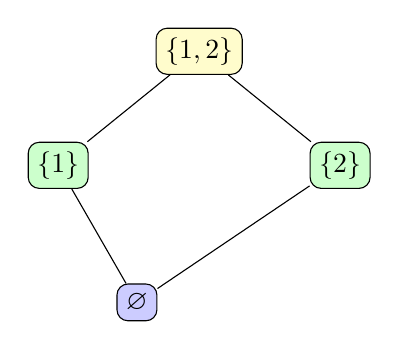
\begin{tikzpicture}[node distance=1.2cm, auto]
  \node[draw, rectangle, rounded corners, fill=yellow!20] (top) {\(\{1,2\}\)};
  \node[draw, rectangle, rounded corners, fill=green!20] (left) [below left=of top] {\(\{1\}\)};
  \node[draw, rectangle, rounded corners, fill=green!20] (right) [below right=of top] {\(\{2\}\)};
  \node[draw, rectangle, rounded corners, fill=blue!20] (bottom) [below=of left, xshift=1cm] {\(\varnothing\)};
  \draw (top) -- (left);
  \draw (top) -- (right);
  \draw (left) -- (bottom);
  \draw (right) -- (bottom);
\end{tikzpicture}
\end{center}

\begin{lemma}
  Every finite, nonempty poset has at least one \emph{minimal} element and at least one \emph{maximal} element.
\end{lemma}

%%%%%%%%%%%%%%%%%%%%%%%%%%%%%%%%%%%%%%%%%%%%%%%%%%%%%%%%%%%%%%%%%%%%%
\subsection{Total Orders and Chains}

\begin{definition}[Total (or Linear) Order]
  A partial order \(\preceq\) on a set \(P\) is a \emph{total order} if for any \(a, b \in P\), either \(a \preceq b\) or \(b \preceq a\).
  \vspace{0.5em}
  \textbf{Why It Matters:} Total orders are used in sorting and scheduling algorithms, as every pair of elements can be compared.
\end{definition}

% Diagram: A chain (total order) illustrated as a straight line
\begin{center}
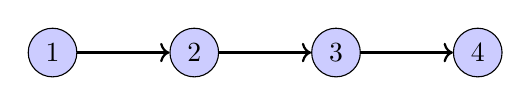
\begin{tikzpicture}[node distance=1.8cm, auto]
  \node[draw, circle, fill=blue!20] (1) {\(1\)};
  \node[draw, circle, fill=blue!20] (2) [right of=1] {\(2\)};
  \node[draw, circle, fill=blue!20] (3) [right of=2] {\(3\)};
  \node[draw, circle, fill=blue!20] (4) [right of=3] {\(4\)};
  \draw[->, thick] (1) -- (2);
  \draw[->, thick] (2) -- (3);
  \draw[->, thick] (3) -- (4);
\end{tikzpicture}
\end{center}

A \emph{chain} in a poset is a subset where every two elements are comparable, while an \emph{antichain} is a subset where no two distinct elements are comparable.

%%%%%%%%%%%%%%%%%%%%%%%%%%%%%%%%%%%%%%%%%%%%%%%%%%%%%%%%%%%%%%%%%%%%%
\subsection{Lattices and Boolean Algebras}

\begin{definition}[Lattice]
  A poset \((L, \preceq)\) is a \emph{lattice} if every pair \(a,b \in L\) has:
  \begin{itemize}[itemsep=3pt]
    \item A unique \emph{least upper bound} (join, \(a \vee b\)).
    \item A unique \emph{greatest lower bound} (meet, \(a \wedge b\)).
  \end{itemize}
  \vspace{0.5em}
  \textbf{Conceptual Insight:} Lattices structure elements in a way that mirrors logical operations, forming the foundation of Boolean algebra.
\end{definition}

\begin{example}
  The power set \(\mathcal{P}(S)\) of any set \(S\), ordered by \(\subseteq\), forms a lattice where:
  \[
  a \vee b = a \cup b \quad \text{and} \quad a \wedge b = a \cap b.
  \]
\end{example}

% Diagram: Lattice diagram (another view of the power set of \{1,2\})
\begin{center}
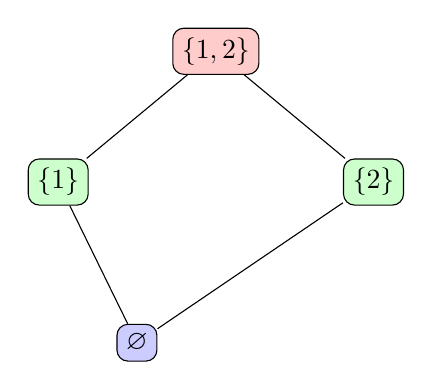
\begin{tikzpicture}[node distance=1.5cm, auto]
  \node[draw, rectangle, rounded corners, fill=red!20] (top) {\(\{1,2\}\)};
  \node[draw, rectangle, rounded corners, fill=green!20] (left) [below left=of top] {\(\{1\}\)};
  \node[draw, rectangle, rounded corners, fill=green!20] (right) [below right=of top] {\(\{2\}\)};
  \node[draw, rectangle, rounded corners, fill=blue!20] (bottom) [below=of left, xshift=1cm] {\(\varnothing\)};
  \draw (top) -- (left);
  \draw (top) -- (right);
  \draw (left) -- (bottom);
  \draw (right) -- (bottom);
\end{tikzpicture}
\end{center}

\begin{lemma}[Distributive Law in Lattices]
  A lattice \(L\) is \emph{distributive} if for all \(a,b,c \in L\):
  \[
  a \wedge (b \vee c) = (a \wedge b) \vee (a \wedge c)
  \]
  and
  \[
  a \vee (b \wedge c) = (a \vee b) \wedge (a \vee c).
  \]
  \vspace{0.5em}
  \textbf{Why It Matters:} Distributivity simplifies computations and underpins Boolean logic.
\end{lemma}

%%%%%%%%%%%%%%%%%%%%%%%%%%%%%%%%%%%%%%%%%%%%%%%%%%%%%%%%%%%%%%%%%%%%%
\subsection{Dilworth's Theorem and Related Results}

Dilworth's Theorem and the Erd\H{o}s--Szekeres Theorem capture deep combinatorial properties, showing that large posets necessarily contain either a long chain or a large antichain.

\begin{theorem}[Dilworth's Theorem]
  In any finite poset, the size of the largest antichain equals the minimum number of chains needed to cover the poset.
  \vspace{0.5em}
  \textbf{Why It Matters:} This theorem is a powerful tool in combinatorics with applications in scheduling and resource allocation.
\end{theorem}

\begin{theorem}[Erd\H{o}s--Szekeres Theorem]
  Any sequence of \(n^2+1\) distinct real numbers contains a monotonic (increasing or decreasing) subsequence of length \(n+1\).
  \vspace{0.5em}
  \textbf{Conceptual Insight:} This result shows that order must emerge in any sufficiently large dataset, an idea that resonates in Ramsey theory.
\end{theorem}

%%%%%%%%%%%%%%%%%%%%%%%%%%%%%%%%%%%%%%%%%%%%%%%%%%%%%%%%%%%%%%%%%%%%%
\section{Combinatorial Counting}

Counting techniques are central to discrete mathematics. They allow us to enumerate possibilities, calculate probabilities, and analyze algorithms.

%%%%%%%%%%%%%%%%%%%%%%%%%%%%%%%%%%%%%%%%%%%%%%%%%%%%%%%%%%%%%%%%%%%%%
\subsection{Counting Functions and Subsets}

\begin{itemize}
  \item The number of functions from a finite set \(A\) (with \(|A| = m\)) to a finite set \(B\) (with \(|B| = n\)) is:
  \[
  n^m.
  \]
  \item The number of injections from \(A\) to \(B\) (when \(m \le n\)) is:
  \[
  P(n, m) = \frac{n!}{(n-m)!}.
  \]
  \item The total number of subsets of an \(n\)-element set is:
  \[
  2^n.
  \]
  \item The number of \(k\)-element subsets is given by the binomial coefficient:
  \[
  \binom{n}{k} = \frac{n!}{k!(n-k)!}.
  \]
\end{itemize}
\vspace{0.5em}
\textbf{Why It Matters:} These formulas form the core of combinatorial reasoning, vital for probability theory and algorithm analysis.

\begin{lemma}[Binomial Sum Identity]
  For any non-negative integer \(n\),
  \[
  \sum_{k=0}^{n} \binom{n}{k} = 2^n.
  \]
\end{lemma}

%%%%%%%%%%%%%%%%%%%%%%%%%%%%%%%%%%%%%%%%%%%%%%%%%%%%%%%%%%%%%%%%%%%%%
\subsection{Permutations and Factorials}

\begin{definition}[Factorial]
  For \(n \in \mathbb{N}\), the \emph{factorial} \(n!\) is defined as:
  \[
  n! = n \cdot (n-1) \cdots 2 \cdot 1, \quad \text{with } 0! = 1.
  \]
\end{definition}

\begin{definition}[Permutation]
  A \emph{permutation} of a set of \(n\) elements is an ordered arrangement. The total number of permutations is \(n!\). More generally, the number of ways to order \(k\) out of \(n\) elements is:
  \[
  P(n,k) = \frac{n!}{(n-k)!}.
  \]
\end{definition}

\begin{lemma}[Permutations with Repetition]
  If there are \(n\) objects with \(n_1\) of one type, \(n_2\) of another, \(\dots\), \(n_k\) of the \(k\)th type (with \(n_1+n_2+\cdots+n_k = n\)), then the number of distinct permutations is:
  \[
  \frac{n!}{n_1!n_2!\cdots n_k!}.
  \]
\end{lemma}

%%%%%%%%%%%%%%%%%%%%%%%%%%%%%%%%%%%%%%%%%%%%%%%%%%%%%%%%%%%%%%%%%%%%%
\subsection{Binomial Coefficients and the Binomial Theorem}

\begin{definition}[Binomial Coefficient]
  For non-negative integers \(n\) and \(k\) with \(0 \le k \le n\), the binomial coefficient is:
  \[
  \binom{n}{k} = \frac{n!}{k!(n-k)!}.
  \]
\end{definition}

\begin{lemma}[Pascal's Identity]
  For \(0 < k < n\),
  \[
  \binom{n}{k} = \binom{n-1}{k-1} + \binom{n-1}{k}.
  \]
  \vspace{0.5em}
  \textbf{Conceptual Insight:} This identity is the backbone of Pascal's Triangle and reveals the recursive structure of binomial coefficients.
\end{lemma}

% Diagram: A small portion of Pascal's Triangle
\begin{center}
\begin{tikzpicture}[node distance=0.8cm, auto]
  \node (row0) {\(1\)};
  \node (row1-1) [below left=of row0] {\(1\)};
  \node (row1-2) [below right=of row0] {\(1\)};
  \node (row2-1) [below left=of row1-1] {\(1\)};
  \node (row2-2) [below=of row0] {\(2\)};
  \node (row2-3) [below right=of row1-2] {\(1\)};
  \draw (row0) -- (row1-1);
  \draw (row0) -- (row1-2);
  \draw (row1-1) -- (row2-1);
  \draw (row1-1) -- (row2-2);
  \draw (row1-2) -- (row2-2);
  \draw (row1-2) -- (row2-3);
\end{tikzpicture}
\end{center}

\begin{theorem}[Binomial Theorem]
  For any real numbers \(x\) and \(y\) and non-negative integer \(n\),
  \[
  (x+y)^n = \sum_{k=0}^{n} \binom{n}{k} x^k y^{n-k}.
  \]
  \vspace{0.5em}
  \textbf{Why It Matters:} The binomial theorem is a powerful tool for expanding expressions and has applications in algebra, probability, and numerical methods.
\end{theorem}

\begin{example}
  For \(n=3\):
  \[
  (x+y)^3 = y^3 + 3xy^2 + 3x^2y + x^3.
  \]
\end{example}

\begin{definition}[Multinomial Coefficients]
  For non-negative integers \(n_1, n_2, \dots, n_k\) satisfying \(n_1+n_2+\cdots+n_k = n\), the multinomial coefficient is:
  \[
  \binom{n}{n_1, n_2, \dots, n_k} = \frac{n!}{n_1!n_2!\cdots n_k!}.
  \]
\end{definition}

\begin{theorem}[Multinomial Theorem]
  For any real numbers \(x_1, x_2, \dots, x_k\) and non-negative integer \(n\),
  \[
  (x_1+x_2+\cdots+x_k)^n = \sum_{n_1+n_2+\cdots+n_k=n} \binom{n}{n_1, n_2, \dots, n_k} \prod_{i=1}^k x_i^{n_i}.
  \]
\end{theorem}

%%%%%%%%%%%%%%%%%%%%%%%%%%%%%%%%%%%%%%%%%%%%%%%%%%%%%%%%%%%%%%%%%%%%%
\subsection{Inclusion-Exclusion Principle}

The inclusion-exclusion principle corrects for over-counting in overlapping sets, a crucial concept in combinatorics.

\begin{theorem}[Inclusion-Exclusion Principle]
  Let \(A_1, A_2, \dots, A_n\) be finite sets. Then:
  \[
  \left| \bigcup_{i=1}^{n} A_i \right| = \sum_{i=1}^{n} |A_i| - \sum_{1\le i < j \le n} |A_i \cap A_j| + \sum_{1\le i < j < k \le n} |A_i \cap A_j \cap A_k| - \cdots + (-1)^{n+1} |A_1 \cap A_2 \cap \cdots \cap A_n|.
  \]
  \vspace{0.5em}
  \textbf{Why It Matters:} This principle is essential for accurately counting elements in overlapping sets.
\end{theorem}

% Diagram: Three-set Venn diagram for Inclusion-Exclusion
\begin{center}
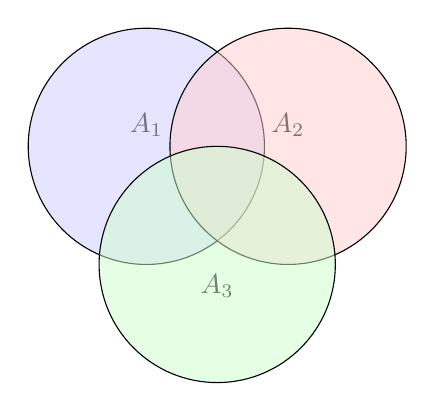
\begin{tikzpicture}
  \draw[fill=blue!20, fill opacity=0.5] (0,0) circle (1.5) node[above] {\(A_1\)};
  \draw[fill=red!20, fill opacity=0.5] (1.8,0) circle (1.5) node[above] {\(A_2\)};
  \draw[fill=green!20, fill opacity=0.5] (0.9,-1.5) circle (1.5) node[below] {\(A_3\)};
\end{tikzpicture}
\end{center}

\begin{example}
  For two sets \(A\) and \(B\):
  \[
  |A \cup B| = |A| + |B| - |A \cap B|.
  \]
\end{example}

%%%%%%%%%%%%%%%%%%%%%%%%%%%%%%%%%%%%%%%%%%%%%%%%%%%%%%%%%%%%%%%%%%%%%
\subsection{Derangements and the Hat-Check Problem}

Derangements are permutations where no element remains in its original position. They provide insight into probability and combinatorial reasoning.

\begin{definition}[Derangement]
  A \emph{derangement} is a permutation \(\sigma\) of \(\{1,2,\dots,n\}\) with \(\sigma(i) \neq i\) for all \(i\).
  \vspace{0.5em}
  \textbf{Why It Matters:} Counting derangements uses inclusion-exclusion and highlights unexpected order in chaos.
\end{definition}

Let \(D_n\) denote the number of derangements of \(n\) objects:
\[
D_n = n! \sum_{k=0}^{n} \frac{(-1)^k}{k!}.
\]
An alternative recurrence is:
\[
D_n = (n-1)(D_{n-1} + D_{n-2}), \quad \text{with } D_0 = 1 \text{ and } D_1 = 0.
\]

\begin{example}
  For \(n=3\):
  \[
  D_3 = 3! \left(1 - \frac{1}{1!} + \frac{1}{2!} - \frac{1}{3!}\right)
  = 6\left(1 - 1 + \frac{1}{2} - \frac{1}{6}\right)
  = 6\left(\frac{1}{3}\right)
  = 2.
  \]
\end{example}

Another useful expression is:
\[
D_n = \left\lfloor \frac{n!}{e} + \frac{1}{2} \right\rfloor,
\]
where \(e\) is the base of the natural logarithm.

%%%%%%%%%%%%%%%%%%%%%%%%%%%%%%%%%%%%%%%%%%%%%%%%%%%%%%%%%%%%%%%%%%%%%
\section*{Conclusion}

In these notes we have explored several core topics in discrete mathematics:
\begin{itemize}
  \item \textbf{Numbers and Sets:} Fundamental structures that underpin all of mathematics.
  \item \textbf{Proof Techniques:} Methods like induction that enable us to rigorously prove infinite families of statements.
  \item \textbf{Functions and Relations:} The language for describing mappings and associations, essential in modeling processes.
  \item \textbf{Ordering:} Concepts such as partial orders, total orders, and lattices that bring structure and hierarchy.
  \item \textbf{Combinatorial Counting:} Techniques to enumerate possibilities, critical in probability and algorithm analysis.
\end{itemize}

These diagrams serve as visual aids to help cement your understanding of the concepts. Feel free to expand on them or adjust as your understanding grows.

\end{document}
